\documentclass[11pt]{article}

% Change "review" to "final" to generate the final (sometimes called camera-ready) version.
% Change to "preprint" to generate a non-anonymous version with page numbers.
\usepackage[review]{acl}

% Standard package includes
\usepackage{times}
\usepackage{latexsym}

% For proper rendering and hyphenation of words containing Latin characters (including in bib files)
\usepackage[T1]{fontenc}
% For Vietnamese characters
% \usepackage[T5]{fontenc}
% See https://www.latex-project.org/help/documentation/encguide.pdf for other character sets

% This assumes your files are encoded as UTF8
\usepackage[utf8]{inputenc}

% This is not strictly necessary, and may be commented out,
% but it will improve the layout of the manuscript,
% and will typically save some space.
\usepackage{microtype}

% This is also not strictly necessary, and may be commented out.
% However, it will improve the aesthetics of text in
% the typewriter font.
\usepackage{inconsolata}

%Including images in your LaTeX document requires adding
%additional package(s)
\usepackage{graphicx}

% For the split environment and other math features
\usepackage{amsmath}
\usepackage{amssymb}

% For algorithms
\usepackage{algorithm}
\usepackage{algorithmic}

% For beautiful table lines (\toprule, \midrule, \cmidrule)
\usepackage{booktabs}
% For dashed lines in tables (\hdashline)
\usepackage{arydshln}
% For multirow cells in tables
\usepackage{multirow}

% If the title and author information does not fit in the area allocated, uncomment the following
%
%\setlength\titlebox{<dim>}
%
% and set <dim> to something 5cm or larger.

\title{CSLF: Mitigating Catastrophic Forgetting via  \\ Cognitive-Semantic and Latent-Feature Collaboration}

% Author information can be set in various styles:
% For several authors from the same institution:
% \author{Author 1 \and ... \and Author n \\
%         Address line \\ ... \\ Address line}
% if the names do not fit well on one line use
%         Author 1 \\ {\bf Author 2} \\ ... \\ {\bf Author n} \\
% For authors from different institutions:
% \author{Author 1 \\ Address line \\  ... \\ Address line
%         \And  ... \And
%         Author n \\ Address line \\ ... \\ Address line}
% To start a separate ``row'' of authors use \AND, as in
% \author{Author 1 \\ Address line \\  ... \\ Address line
%         \AND
%         Author 2 \\ Address line \\ ... \\ Address line \And
%         Author 3 \\ Address line \\ ... \\ Address line}

\author{First Author \\
  Affiliation / Address line 1 \\
  Affiliation / Address line 2 \\
  Affiliation / Address line 3 \\
  \texttt{email@domain} \\\And
  Second Author \\
  Affiliation / Address line 1 \\
  Affiliation / Address line 2 \\
  Affiliation / Address line 3 \\
  \texttt{email@domain} \\}

%\author{
%  \textbf{First Author\textsuperscript{1}},
%  \textbf{Second Author\textsuperscript{1,2}},
%  \textbf{Third T. Author\textsuperscript{1}},
%  \textbf{Fourth Author\textsuperscript{1}},
%\\
%  \textbf{Fifth Author\textsuperscript{1,2}},
%  \textbf{Sixth Author\textsuperscript{1}},
%  \textbf{Seventh Author\textsuperscript{1}},
%  \textbf{Eighth Author \textsuperscript{1,2,3,4}},
%\\
%  \textbf{Ninth Author\textsuperscript{1}},
%  \textbf{Tenth Author\textsuperscript{1}},
%  \textbf{Eleventh E. Author\textsuperscript{1,2,3,4,5}},
%  \textbf{Twelfth Author\textsuperscript{1}},
%\\
%  \textbf{Thirteenth Author\textsuperscript{3}},
%  \textbf{Fourteenth F. Author\textsuperscript{2,4}},
%  \textbf{Fifteenth Author\textsuperscript{1}},
%  \textbf{Sixteenth Author\textsuperscript{1}},
%\\
%  \textbf{Seventeenth S. Author\textsuperscript{4,5}},
%  \textbf{Eighteenth Author\textsuperscript{3,4}},
%  \textbf{Nineteenth N. Author\textsuperscript{2,5}},
%  \textbf{Twentieth Author\textsuperscript{1}}
%\\
%\\
%  \textsuperscript{1}Affiliation 1,
%  \textsuperscript{2}Affiliation 2,
%  \textsuperscript{3}Affiliation 3,
%  \textsuperscript{4}Affiliation 4,
%  \textsuperscript{5}Affiliation 5
%\\
%  \small{
%    \textbf{Correspondence:} \href{mailto:email@domain}{email@domain}
%  }
%}

\begin{document}
\maketitle
\begin{abstract}
Mitigating catastrophic forgetting in continual learning is crucial. Existing methods have made breakthroughs by separating and fine-tuning parameters for different tasks. However, we observe that parameter separation is not truly achieved. The interference among categorical distributions across task-specific models leads to performance degradation as the number of tasks increases. Additionally, their task classification only relies on parameter-level learning, neglecting the model's inherent prior knowledge at semantic level. Inspired by the dual-process theory in cognitive science, we propose a novel architecture: Cognitive-Semantic and Latent-Feature dual-stream synergistic architecture (CSLF), which focuses on achieving correct task classification and true parameter separation. CSLF performs task classification prior to routing samples to task-specific models, avoiding the interference among categorical distributions generated from different task-specific models. Through dynamic task category semantic extraction module and task latent feature abstraction module, CSLF can fully leverage the model's task semantic space and feature mapping space simultaneously. Moreover, an adaptive gated fusion mechanism is integrated in CSLF to better fuse information from both spaces, further improving CSLF's task classification capability. Experiments across various downstream tasks demonstrate the superiority of CSLF, establishing it as a promising paradigm for continual learning by merging semantic and latent features.

\end{abstract}
\section{Introduction}

Continual adaptation is essential for deployed NLP systems, but training on new tasks often overwrites old knowledge and causes catastrophic forgetting~\cite{1,2,3}. Existing solutions include regularization (e.g., EWC~\cite{ewc_2017}), replay~\cite{mem_2022}, and, most effectively in recent LLM settings, parameter separation~\cite{lora,lester2021power,li2021prefix,pre_2024_cor,pre_2022_3}. Although separation reduces direct parameter conflict, current pipelines still suffer from non-trivial cross-task interference.

\begin{figure}[t]
    \centering
    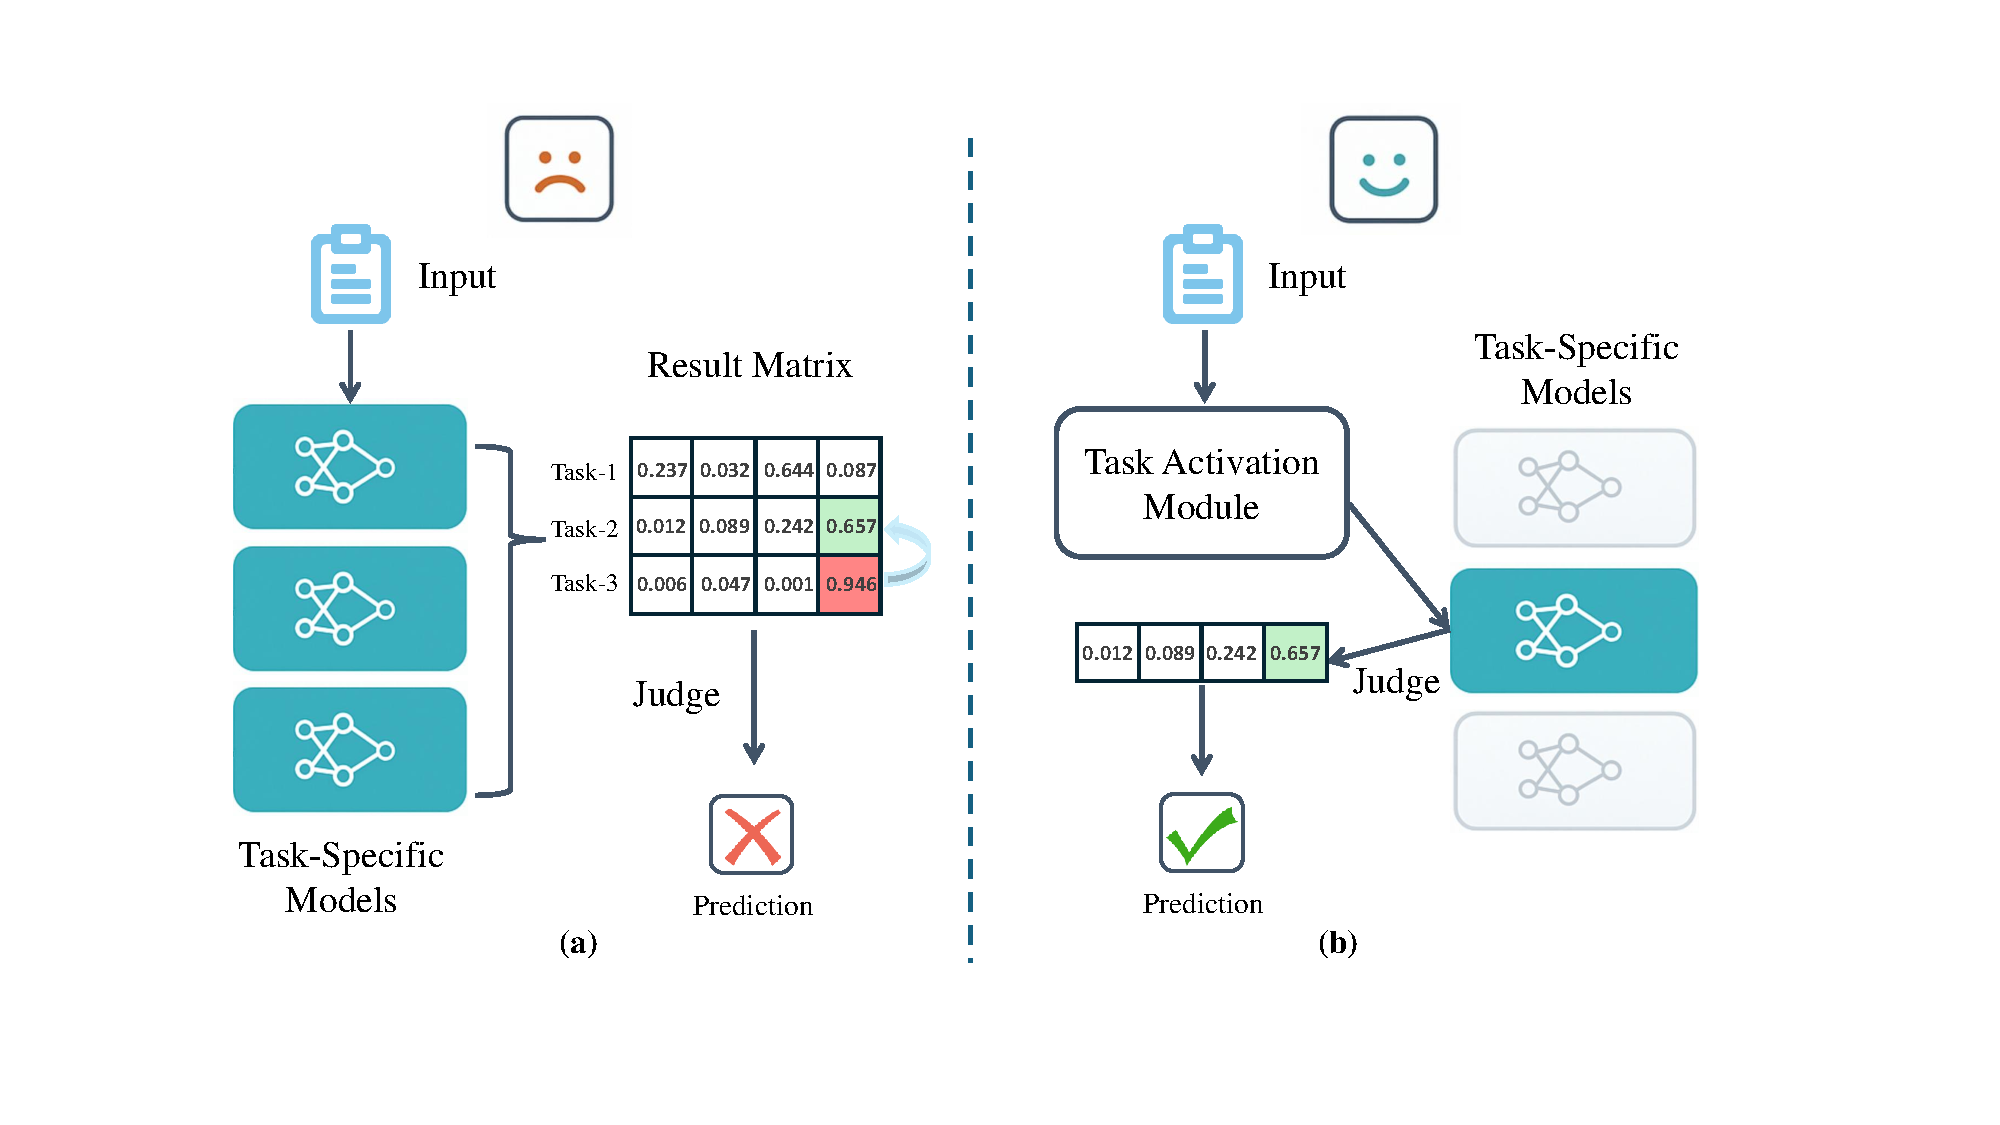
\includegraphics[width=\columnwidth]{main_1.pdf}
    \caption{Right activate Task-Specific models to achieve true parameter isolation.}
    \label{fig:isolation}
\end{figure}

Firstly, samples from different tasks are often processed by multiple task-specific models in parallel, and the final prediction relies on combining outputs from all these models~\cite{164,234,140}. This design leads to inevitable interference among the categorical distributions generated by different separated models, especially as the number of tasks increases~\cite{197}. For instance, when the training process progresses to the third task, where each task introduces four novel subclasses, the final result matrix has a dimension of  3 rows and 4 columns. As illustrated in the Figure~\ref{fig:isolation} (a), the ground truth label of a sample corresponds to the fourth class in the second task (indicated in green). Examining exclusively the output from the task-2 model yields the correct prediction (with 0.657 being the maximum value). However, from a global perspective,  the output value of 0.946 generated by the task-3 model surpasses the optimal solution derived from task-2, thereby introducing interference. The primary reason for this phenomenon is that different task-specific models perform their respective softmax operations individually. Conversely, the human hippocampus first releases neurotransmitters to activate the correct neuronal regions, and only then proceeds to perform complex tasks based solely on the already activated neural circuits~\cite{n1}. Therefore, we first select and activate the right task-specific model and then route samples to the chosen model, as illustrated in the Figure~\ref{fig:isolation} (b).

In addition, current methods primarily perform task classification at the parameter level, overlooking the model's inherent prior knowledge at the semantic level~\cite{175}. In contrast, human cognition adheres to a dual-process principle: the intuitive system and the analytical system. The intuitive system relies on rapid neural electrical signal transmission, characterized by quick responses but low interpretability~\cite{n2,n3}. The analytical system establishes connections between new and existing knowledge through analogical learning at the semantic level. For example, when learning the concept of an ``IP address'', it naturally draws an analogy with a ``postal code'', thereby achieving better learning outcomes. This collaborative mechanism of dual systems ensures both rapid responsiveness and systematic knowledge construction. CSLF architecture draws inspiration from this principle. It dynamically harmonizes semantic knowledge and feature learning, outperforming conventional methods that rely solely on feature space representations. Therefore, our contributions are as follows:

\begin{itemize}
\item We propose a novel framework called the Cognitive-Semantic and Latent-Feature Dual-Stream Synergistic Architecture, which focuses on activating the correct task-specific models, enabling phased decision-making to achieve true parameter isolation and avoid interference between different tasks.
\item Building upon the dual-process cognitive theory, we design key components, including a dynamic task category semantic extraction module and a task latent feature abstraction module. Our framework is the first to  synergistically combine semantic knowledge with feature learning in the field of continual learning. It uniquely incorporates prior knowledge from large language model pretraining into continual learning paradigms.

\item We design an adaptive gated fusion mechanism to  fully and efficiently fuse information from the two spaces, facilitating accurate
and dynamic activation of task-specific models. Extensive experiments on multiple downstream tasks and comprehensive analyses demonstrate the superior performance of CSLF.
\end{itemize}


\begin{figure*}[t]
    \centering
    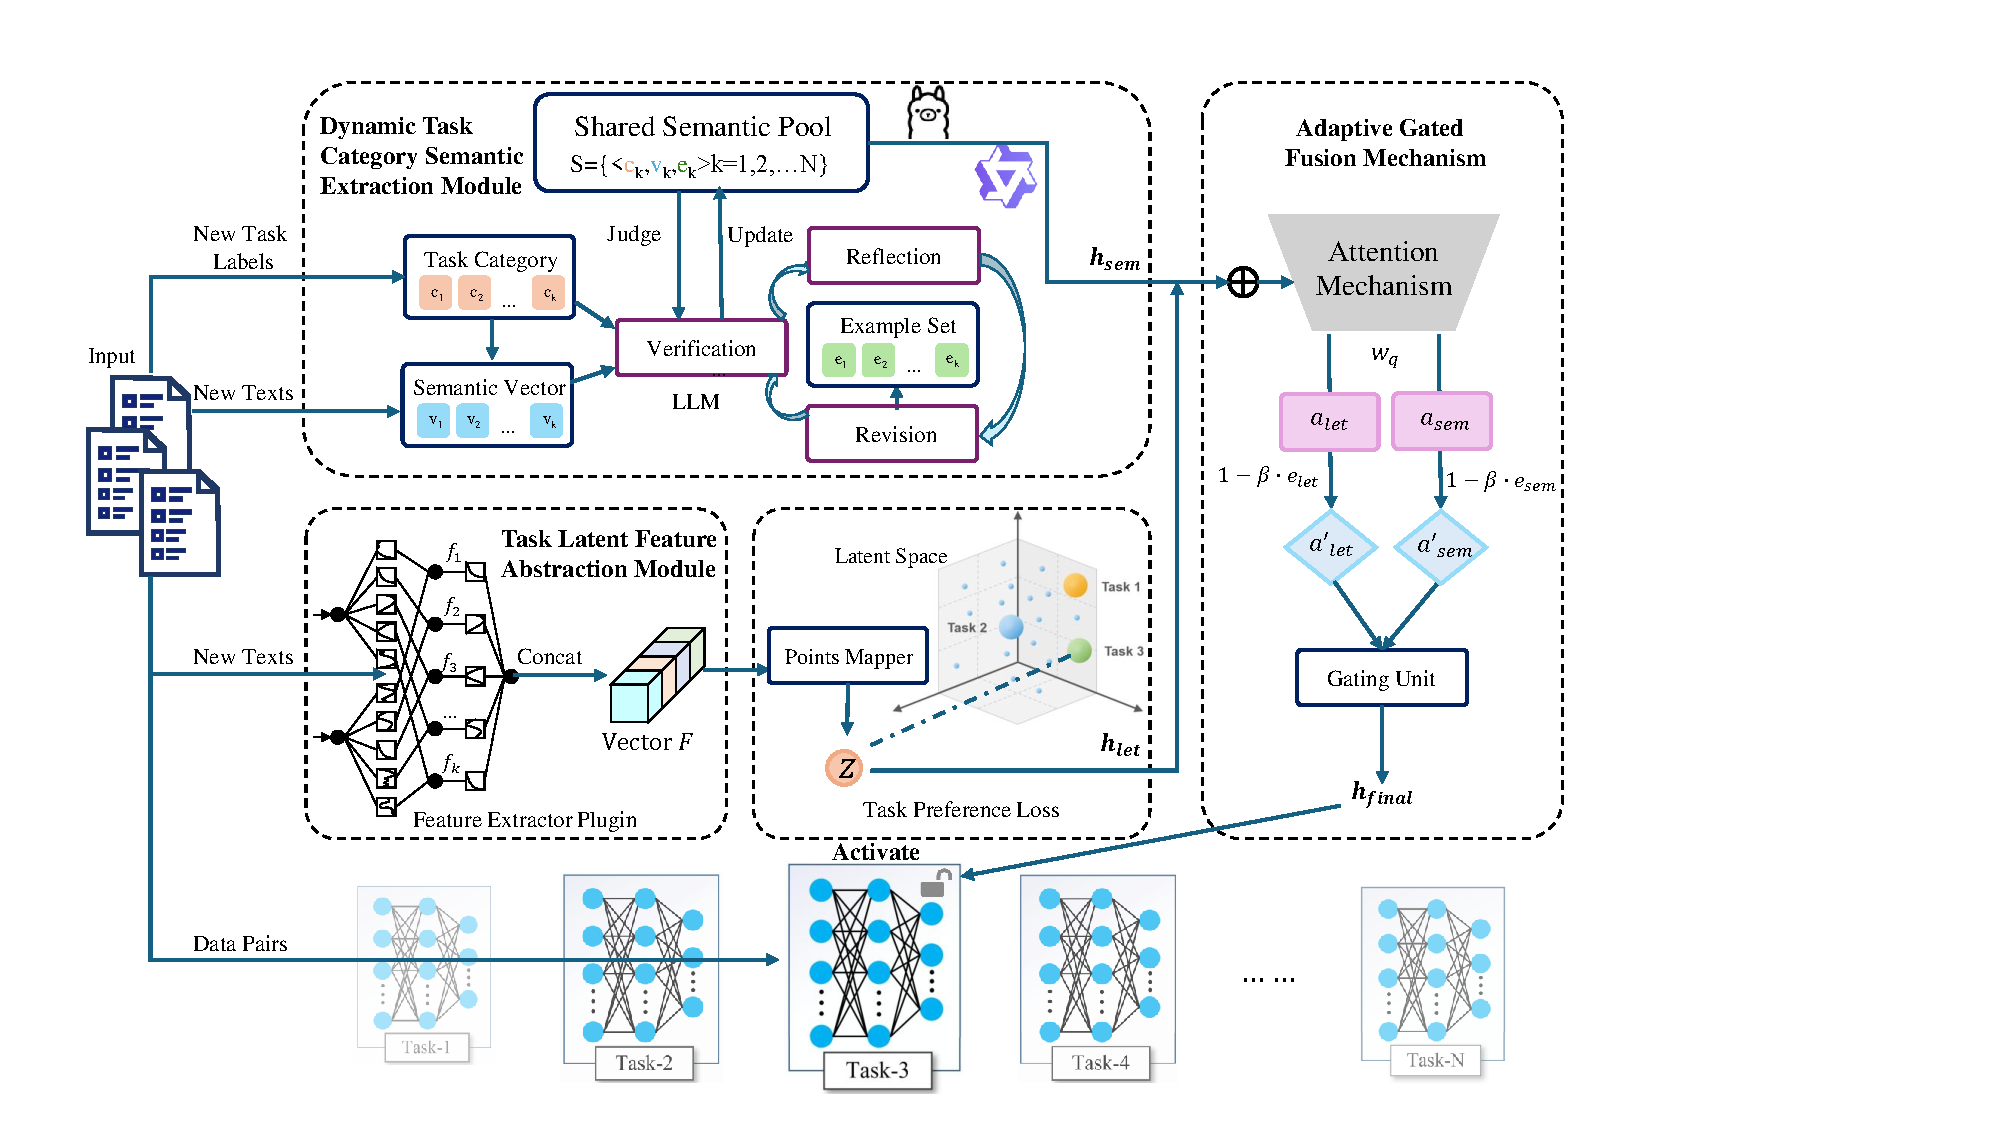
\includegraphics[width=0.85\textwidth]{main_2.pdf}
    \caption{Complete Architecture of CSLF Framework showing the interaction between semantic extraction, latent feature processing, and adaptive fusion mechanisms.}
    \label{fig:framework}
\end{figure*}

\section{Related Work}

\subsection{Continual Learning}

Traditional methods training large language models (LLMs) on static datasets struggle with dynamic real-world information~\cite{brown2020language,tonmoy2024comprehensivesurveyhallucinationmitigation}. Continual learning~\cite{rw2} enables continuous adaptation~\cite{rw3}, but faces the core challenge of catastrophic forgetting when integrating new knowledge. Existing solutions mainly fall into three categories. Regularization methods~\cite{chen2020recall,liu2023class} penalize updates to previously critical weights, though inaccurate weight estimation can hinder new learning. Replay methods reinforce prior knowledge via historical data~\cite{liu2021domain} or generated samples~\cite{qin2021lfpt5}, which introduces privacy and storage overhead issues~\cite{huang2024mitigating}. In contrast, architecture-based methods~\cite{zheng2024beyond} leverage parameter-efficient fine-tuning to add new components or separate parameters for different tasks, achieving notable success in continual learning.

\subsection{Methods Based on Parameter Separation}
Parameter separation~\cite{wang2023orthogonal,wistuba2023continual} is a crucial architecture-based approach in continual learning that effectively minimizes task interference. Furthermore, for massive models like LLaMA-65B~\cite{touvron2023llama} and GLM-130B~\cite{zeng2022glm}, it avoids the prohibitive cost of full-parameter fine-tuning. We briefly overview two prominent separation methods. First, Adapters~\cite{houlsby2019parameter} insert lightweight bottleneck feed-forward networks between layers for efficient task adaptation, with variants like LAFT-URIEL~\cite{badola2022parameter} and TSS~\cite{ke2023sub} enhancing them via feature guidance and soft-masking. Second, LoRA~\cite{lora} integrates trainable low-rank matrices into pre-trained layers for parameter-efficient updates. Frameworks like CoLoR~\cite{wistuba2023continual} adopt LoRA for continual learning, while subsequent works~\cite{i_lora,inf_lora} further incorporate enhancements like data replay.

\section{Methodology}
Given a series of  tasks $ T_1, \ldots, T_N $, where the total number of tasks is $ N $, each task  $ T_i $ introduces $ G $ new classes $ Y_i = \{Y_i^1, \ldots,Y_i^g \ldots,Y_i^G\} $. Each new class contains $ h $ labeled examples, represented as data pairs $ (x_{i,g}^{j}, y_{i,g}^{j},j=1, \ldots, h) $.  The learner's objective is to learn or optimize the current parameters $ \Theta $ such that the average categorical loss across all tasks, $ \frac{1}{N} \sum_{i \in \{1, \ldots, N\}} \mathcal{L}(T_i; \Theta) $, is minimized. The challenge of continual learning lies in the fact that these tasks cannot be learned all at once, but must be acquired one by one.

The framework of the proposed CSLF architecture is illustrated in Figure~\ref{fig:framework}. The architecture consists of three main modules: Dynamic Task Category Semantic Extraction Module, Task Latent Feature Abstraction Module, and adaptive Gated Fusion Mechanism to integrate both signals for task routing~\cite{attention,bahdanau2014neural}.

Our framework handles multiple tasks where each task requires learning new class categories. At the start of task $T_t$, we inject its new class labels into the semantic stream and attach a unique task ID $t$ to the corresponding task-specific adapter. The semantic stream produces a task-activation vector from category semantics and a prompted backbone prediction, while the latent stream produces another activation vector from intermediate hidden states. The two vectors have the same dimensionality as the number of observed tasks and are fused before selecting the activated task-specific model. Importantly, the semantic stream is used as a non-differentiable routing signal, whereas the latent stream is trained end-to-end with the active task adapter and the points mapper. This division avoids backpropagating through discrete prompting decisions while preserving a fully trainable latent routing path. Detailed prompts, tensor shapes, and optimization behavior are provided in Appendix~H.

\subsection{Dynamic Task Category Semantic Extraction Module}

This module maintains a shared semantic pool $\mathcal{S} = \{ \langle \mathbf{c}_k, \mathbf{v}_k, \mathbf{e}_k \rangle \mid k = 1, 2, \dots, N \}$, where $\mathbf{c}_k$ denotes the label texts associated with task $k$, $\mathbf{v}_k \in \mathbb{R}^{384}$ is the MiniLM embedding of the task description, and $\mathbf{e}_k \subseteq \mathcal{D}_k$ is a small exemplar buffer used to refine the task description. Each entry points to a unique task ID rather than to a fine-grained class ID, because the goal of this module is routing across task-specific adapters.

\subsubsection{Dynamic Category Semantic Extraction.}

When a new task arrives, its categories $\mathbf{c}_{\text{new}} = \{ c_{K+1}, \dots, c_{K+g} \}$ are dynamically injected into the semantic pool. The initial semantic vector for each new category is computed as
\begin{equation}
    \mathbf{v}_{K+i} = \text{Embedding}(c_{K+i}), \quad i = 1, \dots, g
\end{equation}
where Embedding is achieved through a light embedding model MiniLM-L12-v2.

This enables the model to maintain global category awareness. At the semantic level, the one-to-one correspondence between the model ID and the semantics of the categorical labels is established.


\subsubsection{Similarity Calculation and Iterative Verification.}

For a training batch $\mathcal{B} = \{ x_1, \dots, x_N \}$, we compute the similarity between each sample and the semantic vectors in the pool. This is done by calculating the cosine similarity~\cite{lahitani2016cosine}:
\begin{equation}
    \text{Sim}(x_i, \mathbf{v}_k) = \frac{\text{Embedding}(x_i) \cdot \mathbf{v}_k}{\|\text{Embedding}(x_i)\|_2 \|\mathbf{v}_k\|_2} 
\end{equation}

Let $\mathbf{s}_i = [\text{Sim}(x_i,\mathbf{v}_1), \ldots, \text{Sim}(x_i,\mathbf{v}_{|\mathcal{S}|})] \in \mathbb{R}^{|\mathcal{S}|}$ denote the similarity vector. We then build a prompted routing query by concatenating: (1) the input text $x_i$, (2) the top-$m$ nearest task descriptions ranked by $\mathbf{s}_i$, and (3) at most $b$ stored exemplars per candidate task. The backbone LLM is asked to output one task ID from the current candidate set. Concretely, $\text{Backbone}(x_i,\text{Sim}(x_i,\mathbf{v}_k))$ denotes this prompted forward pass and returns a task-score vector $\mathbf{h}_{i} \in \mathbb{R}^{|\mathcal{T}_{\le t}|}$ over the observed tasks:

\begin{equation}
   \mathbf{h}_{i} = \text{Backbone}(x_i,\text{Sim}(x_i, \mathbf{v}_k)) 
\end{equation}
The score vector is obtained from the normalized log-probabilities of the candidate task-ID strings. This semantic routing step uses the generative backbone only in forward mode, is not differentiated, and does not receive gradient updates from the routing loss. However, for entirely novel categories or fine-grained subcategories not encountered during pretraining, its performance tends to degrade. To address this, we employ an iterative verification-reflection-revision mechanism.

The system evaluates the activation accuracy as follows:
\begin{equation}
j^* = \arg\max_j \textbf{h}_i[j], \quad r_i = 
\begin{cases} 
1, & \text{if } j^* = k, \\
0, & \text{otherwise.}
\end{cases}
\end{equation}


The average of all samples in this batch is then calculated.
\begin{equation}
    \bar{r} = \frac{1}{|\mathcal{B}|} \sum_{x_i \in \mathcal{B}} r_i
\end{equation}

\subsubsection{Reflection and Revision.}

If $\bar{r}$ falls below the threshold, we revise the semantic pool with a deterministic reflection procedure. Specifically, we collect the misrouted samples in the current batch, group them by predicted/true task pair, retain the top-$b$ highest-confidence errors per pair, and append them to the exemplar buffers $\mathbf{e}_k$. We then rebuild the task description by prompting the backbone to summarize: (1) the shared topic within each task, (2) the boundary to the most frequently confused neighboring task, and (3) short lexical cues extracted from the retained exemplars. The complete prompt template and update rules are reported in Appendix~H. This loop improves semantic routing without changing the backbone parameters.



Our approach ensures fine-grained category representation accuracy through continuous evolution of the semantic pool
\begin{equation}
    \mathcal{S}' = \mathcal{S} \cup \{ \langle\mathbf{c}_{K+i}, \mathbf{v}_{K+i}, \mathbf{e}_{K+i} \rangle \}
\end{equation}


In the inference stage, the backbone obtains the semantic-space activation vector $\mathbf{h}_{sem} \in \mathbb{R}^{|\mathcal{T}_{\le t}|}$ based on the updated semantic pool $\mathcal{S}'$.

\begin{equation}
    \mathbf{h}_{sem} = \text{Backbone}(\mathcal{S}', x_i)
\end{equation}

For any input sentence $x_i$, the module outputs a semantic-space activation vector $\mathbf{h}_{sem}$. For a detailed overview of the training process, please refer to Algorithm 1.
\begin{algorithm}[t]
\caption{Dynamic Task Category Semantic Extraction Module}
\begin{algorithmic}[1]
\REQUIRE Existing semantic pool $\mathcal{S}$, new task categories $\mathbf{c}_{\text{new}} = \{c_{K+1}, \dots, c_{K+g}\}$, training batch $\mathcal{B}$
\ENSURE Updated semantic pool $\mathcal{S}'$, semantic activation vector $\mathbf{h}_{sem}$

\FOR{each $c_{K+i} \in \mathbf{c}_{\text{new}}$}
    \STATE Compute semantic vector: $\mathbf{v}_{K+i}$ via equation (1)
    \STATE Initialize representative samples: $\mathbf{e}_{K+i} = \emptyset$
\ENDFOR


\FOR{each $x_i \in \mathcal{B}$}
    \FOR{each $\mathbf{v}_k \in \mathcal{S}'$}
        \STATE Compute similarity: $\text{Sim}(x_i, \mathbf{v}_k)$ via equation (2)
    \ENDFOR
    \STATE Get initial activation: $\mathbf{h}_i$ via equation (3) 
\ENDFOR

\STATE Evaluate activation accuracy for batch $\mathcal{B}$
\FOR{each $x_i \in \mathcal{B}$}
    \STATE compute single sample accuracy via equation (4)
\ENDFOR
\STATE Compute average accuracy via equation (5)

\WHILE{$\bar{r} < \tau$}
    \STATE Perform reflection and revision:
    \STATE \quad Record misclassified samples and update $\mathbf{e}_{K+i}$
    \STATE Update semantic pool $\mathcal{S}'$ via equation (6)
    \STATE Recompute activation and accuracy $\bar{r}$
\ENDWHILE

\STATE $\mathbf{h}_{sem} = \text{Backbone}(\mathcal{S}', x_i)$
\STATE \textbf{return} Updated semantic pool $\mathcal{S}'$, semantic activation vector $\mathbf{h}_{sem}$

\end{algorithmic}
\end{algorithm}

\subsection{Task Latent Feature Abstraction Module}




Semantic routing can be unreliable when prior knowledge is weak. We therefore add a latent-feature stream for complementary task discrimination.



Specifically, the input text is fed into the active backbone together with the current task adapter. We extract hidden states from four evenly spaced intermediate layers (layers 6, 12, 18, and 24 for 24-layer backbones; for backbones with a different depth, we use the closest quartile layers). From each selected layer we apply mean pooling over the non-padding tokens to obtain $\mathbf{f}_i \in \mathbb{R}^{d_{\text{hid}}}$. For token-level tasks, mean pooling is restricted to the marked entity span. The composite feature representation is then built by concatenation:
\begin{equation}
\mathbf{F} = \text{Concat}(\mathbf{f}_{1}, \mathbf{f}_{2}, \dots, \mathbf{f}_{k}) \in \mathbb{R}^{\sum_{i=1}^k d_{i}}
\end{equation}
where $k=4$, $d_i=d_{\text{hid}}$, and $\text{Concat}(\cdot)$ denotes feature concatenation. The resulting vector $\mathbf{F} \in \mathbb{R}^{4d_{\text{hid}}}$ retains both shallow and deep signals.

These fused features $\mathbf{F}$ are then input into the points mapper. Let the mapping function of this points mapper be $\mathcal{M}: \mathbb{R}^D \to \mathbb{R}^H$ ($D = 4d_{\text{hid}}$ and $H = 256$). In practice, $\mathcal{M}$ is a two-layer MLP with dimensions $D \rightarrow 512 \rightarrow 256$, GELU activation, and LayerNorm after each linear projection. The mapped feature is:
\begin{equation}
\mathbf{z} = \mathcal{M}(\mathbf{F}) \in \mathbb{R}^H
\end{equation}
In this high-dimensional vector space $\mathbb{R}^H$, each task $T$ is assigned a unique coordinate position $\mathbf{p}_T \in \mathbb{R}^H$. A new point is created whenever a new task arrives. All task points are learnable, initialized from $\mathcal{N}(0, 0.02^2)$, and jointly optimized with $\mathcal{M}$ and the active task adapter.

To enhance task discrimination, we introduce a task preference loss $\mathcal{L}_{\text{task}}$ that uses the known training task ID as supervision. It optimizes the feature representation $\mathbf{z}$ of the current task $T$ to be close to the coordinate point $\mathbf{p}_T$ while being far from the points $\mathbf{p}_{T'}$ of other tasks $T' \in \mathcal{T} \setminus \{T\}$:
\begin{equation}
\begin{split}
\mathcal{L}_{\text{task}} = 
& \underbrace{\|\mathbf{z} - \mathbf{p}_T\|_2^2}_{\text{attraction}} \\
& + \lambda \cdot \underbrace{\sum_{T' \in \mathcal{T} \setminus \{T\}} \max(0, \gamma - \|\mathbf{z} - \mathbf{p}_{T'}\|_2^2)}_{\text{repulsion}}
\end{split}
\label{eq:task-loss}
\end{equation}
where $\|\cdot\|_2^2$ is the squared Euclidean distance, $\lambda > 0$ is the weight of the repulsion term, and $\gamma > 0$ is the minimum margin threshold. By minimizing this loss:
\begin{equation}
\min_{\theta,\{\mathbf{p}_T\}} \mathcal{L}_{\text{task}}
\end{equation}
where $\theta$ are the learnable parameters of the points mapper, we obtain supervised task-ID separation in latent space. We emphasize this point because the loss requires the current sample's task membership during training; therefore it should be understood as a supervised auxiliary routing loss rather than an unsupervised separation objective.

The distances from the mapped feature to all task points are calculated as follows:
\begin{equation}
    \mathbf{d_{T}} = \|\mathbf{z} - \mathbf{p}_{\mathcal{T}}\|_2^2
\end{equation}
The latent feature space activation vector $\mathbf{h}_{lat} \in \mathbb{R}^{|\mathcal{T}_{\le t}|}$ is then derived by inverse min-max normalization on $\mathbf{d_{T}}$, so smaller distances correspond to larger routing scores.

\subsection{Adaptive Gated Fusion Mechanism}




Semantic and latent streams provide complementary activations with input-dependent reliability. We use attention with error-aware correction to reweight them online.

First,  $\mathbf{h}_{sem}$ and $\mathbf{h}_{lat}$ are concatenated into a fused feature $\mathbf{h}_{concat} = [\mathbf{h}_{sem}; \mathbf{h}_{lat}]$, which serves as the input to the scorer. Then, compute the attention weights by introducing a learnable attention query vector $\mathbf{w}_q$ and calculating the attention for each vector via inner product:

\begin{equation}
\begin{split}
    \left[ \alpha_{sem}, \alpha_{lat} \right] &= \text{softmax}\left(\left[ \mathbf{w}_q^\top \cdot \mathbf{h}_{sem}, \mathbf{w}_q^\top \cdot \mathbf{h}_{lat} \right]\right)
\end{split}
\label{eq:joint-attention}
\end{equation}

where $\alpha_{sem}$ and $\alpha_{lat}$ are the initial weights for the semantic and latent feature spaces, respectively, satisfying $\alpha_{sem} + \alpha_{lat} = 1$.

To avoid mismatches between initial attention weights and their real-world activation performance, we introduce an \textbf{error feedback correction term}. During training, the activation error rates of the two vectors, denoted as $e_{sem}$ and $e_{lat}$, are tracked. The corrected weights are computed as:
\begin{equation}
\begin{split}
    \alpha'_{sem} = \alpha_{sem} \cdot (1 - \beta \cdot e_{sem}) \\
    \quad \alpha'_{lat} = \alpha_{lat} \cdot (1 - \beta \cdot e_{lat})
    \label{eq:error-correction}
\end{split}
\end{equation}
where $\beta \in (0,1)$ is the error penalty coefficient, ensuring that vectors with higher error rates have their weights significantly reduced (e.g., if the semantic space activation has more errors, $e_{sem}$ increases and $\alpha'_{sem}$ is automatically attenuated). Based on the corrected weights $\alpha'_{sem}$ and $\alpha'_{lat}$, the final activation vector is generated via a gating unit:
\begin{equation}
    \mathbf{h}_{final} = \alpha'_{sem} \cdot \mathbf{h}_{sem} + \alpha'_{lat} \cdot \mathbf{h}_{lat}
    \label{eq:gated-fusion}
\end{equation}

The core function of the gating unit is to achieve ``dynamic selection'' rather than simple weighting: when the error rate of one space remains high (e.g., $e_{sem} \to 1$), its weight $\alpha'_{sem} \to 0$, and the final output approximates the latent feature space vector; conversely, if the latent space is less reliable, the output emphasizes the semantic space vector. This realizes an ``adaptive winner-takes-most'' adjustment.

$\mathbf{h}_{final}$ is then used for the final classification task, where the task-specific model ID is determined by the maximum value in the vector:
\begin{equation}
    \text{Model ID} = \arg\max_i \mathbf{h}_{final}[i]
\end{equation}
During the inference phase, the task-specific model ID for the current sample is first determined using $\mathbf{h}_{final}$. The sample is then routed to the corresponding task-specific model for prediction, yielding the final classification result.




\section{Experiments}


\subsection{Experimental Settings}

\begin{table*}[t]
\centering

\begin{tabular}{lcccccccc}
\toprule
\multirow{2}{*}{Model} & 
\multicolumn{2}{c}{Banking77} & 
\multicolumn{2}{c}{FewRel} & 
\multicolumn{2}{c}{Few-NERD} & 
\multicolumn{2}{c}{CLINC150} \\
\cmidrule(r){2-3} \cmidrule(r){4-5} \cmidrule(r){6-7} \cmidrule(r){8-9}
& $Score_{N-1}$  & $Score_{N}$ & $Score_{N-1}$ & $Score_{N}$ & $Score_{N-1}$ & $Score_{N}$ & $Score_{N-1}$ & $Score_{N}$ \\
\midrule
\multicolumn{9}{c}{Llama-3-8B} \\
\midrule
SEQ & 15.98 & 14.28 & 13.23 & 9.64 & 10.86 & 9.25 & 7.14 & 6.67 \\
EWC  & 40.41 & 38.40 & 32.25 & 29.18 & 37.84 & 33.02 & 48.03 & 45.39 \\
DER++  & 51.16 & 49.82 & 49.21 & 47.90 & 48.63 & 47.21 & 49.67 & 48.33 \\
\hdashline 
DMEA  & 60.20 & 58.91 & 67.75 & 65.41 & 64.12 & \underline{62.97} & \underline{70.02} & \underline{68.88} \\
InfLoRA & \underline{67.81} & \underline{63.32} & 65.04 & 61.93 & \underline{65.32} & 60.12 & 68.32 & 64.20 \\
I-LoRA & 65.44 & 61.03 & \textbf{71.34} & \underline{68.82} & 62.89 & 59.73 & 61.31 & 60.16 \\
\hdashline 
CSLF(Ours) & \textbf{75.12} & \textbf{74.01} & \underline{70.44} & \textbf{69.38} & \textbf{72.67} & \textbf{69.55} & \textbf{78.83} & \textbf{75.74} \\
\midrule
\multicolumn{9}{c}{Qwen-3-14B} \\
\midrule
SEQ & 17.45 & 15.12 & 15.23 & 11.21 & 10.31 & 8.97 & 9.02 & 8.55 \\
EWC  & 41.67 & 39.88 & 36.41 & 32.85 & 39.12 & 34.28 & 49.23 & 47.01 \\
DER++  & 53.12 & 51.34 & 51.09 & 49.82 & 50.56 & 49.18 & 52.13 & 50.97 \\
\hdashline 
DMEA  & 62.89 & 60.41 & 63.02 & 61.77 & 64.01 & 62.62 & \underline{75.01} & \underline{72.88} \\
InfLoRA & 68.81 & 67.12 & 66.23 & 64.91 & 65.12 & 63.73 & 66.12 & 64.94 \\
I-LoRA & \underline{70.03} & \underline{68.87} & \underline{71.01} & \underline{69.62} & \underline{71.09} & \underline{69.41} & 71.21 & 69.98 \\
\hdashline 
CSLF(Ours) & \textbf{78.21} & \textbf{75.18} & \textbf{72.12} & \textbf{70.93} & \textbf{73.23} & \textbf{71.98} & \textbf{82.01} & \textbf{80.77} \\
\bottomrule
\end{tabular}
\caption{Performance comparison of different methods on four continual learning datasets. The $Score_{N-1}$ represents the average accuracy when training up to the second-to-last task, and the $Score_{N}$ represents the average accuracy when training up to the last task. The best results are in \textbf{bold}, and the second-best results are underlined.}
\label{tab:main-results}
\end{table*}

We conduct extensive experiments to evaluate the performance of the CSLF framework across various downstream tasks. 

\subsubsection{Datasets.} To comprehensively evaluate the effectiveness and generalizability of CSLF, we conduct experiments on four widely-used benchmark datasets spanning diverse downstream tasks: intent recognition, relation extraction, named entity recognition, and text classification. Specifically, we use Banking77~\cite{casanueva2020efficient} for intent detection in the banking domain , FewRel~\cite{han2018fewrel} for relation extraction (80 classes, 8 tasks, 10 classes per increment), Few-NERD~\cite{ding2021few} for fine-grained named entity recognition (66 classes, 11 tasks, 6 classes per increment), and CLINC150~\cite{ethayarajh2019contextual} for multi-domain text classification (150 classes, 15 tasks, 10 classes per increment). This broad selection covers both sentence-level and token-level continual learning scenarios, ensuring a thorough and robust assessment of CSLF across a wide range of real-world applications.

\subsubsection{Baselines.} We compare CSLF with several strong baselines, including classic regularization-based and replay-based methods, as well as the latest parameter separation approaches. Parameter separation is mainly implemented via Adapters and LoRA techniques, establishing a more comprehensive comparison framework.

SEQ (Sequential Fine-tuning) serves as the lower bound for continual learning performance; EWC~\cite{ewc_2017}, a classic regularization-based method, mitigates forgetting by selectively slowing down the learning of weights important for previous tasks; DER++~\cite{derpp}, a representative replay-based method, maintains performance by replaying stored samples from previous tasks; DMEA~\cite{dmea} implements task-specific parameter separation using the Adapter technique; InfLoRA~\cite{inf_lora} achieves parameter separation via LoRA, originally proposed for vision tasks, and we re-implement it for NLP tasks; I-LoRA~\cite{i_lora} combines data replay and LoRA-based parameter separation to improve continual learning.
\subsubsection{Implementation Details.}  CSLF is trained on a single NVIDIA A100 GPU with 80GB memory. The training batch size is set from 4 to 16, and the learning rate is initialized at 1e-5. The task-specific model employs LoRA for efficient parameter adaptation. The rank of LoRA is 4, the scaling factor is 8, and the dropout rate is 0.1. In the semantic stream, MiniLM-L12-v2 is used only for 384-dimensional similarity retrieval, and the backbone LLM is queried with a fixed routing prompt to produce task-ID scores without gradient updates. In the latent stream, the backbone forward pass is differentiated through the active LoRA adapter, while the frozen backbone weights remain unchanged. We extract hidden states from four intermediate layers, mean-pool them, concatenate them, and map them to a 256-dimensional routing space with a two-layer MLP. For fairness, all compared methods are additionally evaluated under multiple random seeds and multiple task orders, and we report significance testing in Appendix~H.6. Additional prompt templates and optimization details are given in Appendix~H.



\subsubsection{Backbone.} We use the Llama-3-8b model~\cite{grattafiori2024llama3herdmodels} and Qwen3-14B model~\cite{qwen3} as the backbone for CSLF. These models are chosen for their strong performance in various NLP tasks and their ability to handle large-scale data efficiently. The models are pre-trained on extensive corpora, providing a solid foundation for continual learning.

\subsubsection{Evaluation Metrics.} We evaluate model performance using three standard metrics:

\textbf{Average Accuracy (AA)} measures the final mean accuracy across all tasks:
\begin{equation}
    AA = \frac{1}{N} \sum_{i=1}^{N} Acc(i, N)
\end{equation}
where $Acc(i, N)$ is the accuracy on task $i$ after learning all $N$ tasks.

\textbf{Backward Transfer (BWT)} quantifies how new learning affects prior tasks (negative values indicate forgetting):
\begin{equation}
    BWT = \frac{1}{N-1} \sum_{i=1}^{N-1} \left[ Acc(i, N) - Acc(i, i) \right]
\end{equation}

\textbf{Forward Transfer (FWT)} evaluates how prior knowledge facilitates learning of new tasks:
\begin{equation}
    FWT = \frac{1}{N-1} \sum_{j=2}^{N} \left[ Acc(j, j-1) - Acc_{scratch}(j) \right]
\end{equation}


\subsection{Main Results}
As shown in Table~\ref{tab:main-results}, CSLF delivers superior performance across all benchmarks. On CLINC150, it achieves 78.83\%/75.74\%, significantly outperforming the top baseline (70.02\%/68.88\%). For Banking77, CSLF exceeds the second-best method by over 7\%. Similarly, it yields state-of-the-art results on FewRel (70.44\%/69.38\%) and Few-NERD (72.67\%/69.55\%). This demonstrates that CSLF mitigates catastrophic forgetting while retaining high adaptability. 

\begin{table}[ht]
    
    \centering
    \begin{tabular}{lcc}
        \toprule
        Method & BWT  & FWT  \\
        \midrule
        SEQ & -43.28 & 10.13 \\
        EWC & -6.34 & 12.32 \\
        DER++ & -8.38 & 13.46 \\
        \hdashline
        DMEA & -4.24 & 13.57 \\
        InfLoRA & -3.25 & 15.13 \\
        I-LoRA & -3.47 & 16.25 \\
        \hdashline
        \textbf{CSLF (Ours)} & \textbf{-2.74} & \textbf{16.82} \\
        \bottomrule
        
    \end{tabular}
    \caption{BWT (Backward Transfer) and FWT (Forward Transfer) results of CSLF and baseline methods on Llama-3-8B model.}
    \label{tab:transfer-results}
    
\end{table}



These consistent improvements across Llama-3-8B and Qwen-3-14B highlight CSLF's robustness. The gating mechanism dynamically balances semantic priors and latent features, achieving true parameter isolation against cross-task interference.

Table~\ref{tab:transfer-results} presents BWT and FWT results on Llama-3-8B. While regularization (EWC, DER++) and separation methods (DMEA, I-LoRA) alleviate SEQ's severe forgetting, CSLF achieves optimal performance—minimizing forgetting and maximizing new gains—validating its effectiveness.

\subsection{Ablation Study and Analysis}

To evaluate the components of CSLF, we conducted ablation studies on the Banking77 dataset (Table~\ref{tab:ablation}). Results show that the semantic component effectively leverages inherent knowledge for task classification, while the latent feature component provides complementary information. Specifically, the semantic module alone yields significant improvements over baselines, highlighting the value of pre-trained knowledge, whereas the latent module excels in capturing abstract boundaries. Combining both components significantly improves performance, suggesting they capture orthogonal task characteristics. Furthermore, adding the attention mechanism enables dynamic weighting for better classification. The error-aware gating mechanism enhances adaptability by suppressing unreliable signals and selecting the most reliable stream. The full CSLF framework achieves the best performance, demonstrating synergistic benefits.



\begin{table}[ht]
    \centering
    \begin{tabular}{lccc}
        \toprule
        Components & AA  & BWT  & $\Delta$AA \\
        \midrule
        \multicolumn{4}{c}{\textit{Baselines}} \\
        \midrule
        SEQ & 15.98 & -44.09 & - \\
        I-LoRA & 65.44 & -3.03 & +49.46 \\
        \midrule
        \multicolumn{4}{c}{\textit{CSLF Components}} \\
        \midrule
        Semantic (S) & 58.23 & -8.45 & +42.25 \\
        Latent (L) & 52.17 & -12.34 & +36.19 \\
        S + L (Simple) & 67.89 & -5.21 & +51.91 \\
        + Attention & 70.45 & -4.12 & +54.47 \\
        + Gating & 72.78 & -3.67 & +56.80 \\
        \midrule
        \textbf{CSLF (Full)} & \textbf{75.12} & \textbf{-2.74} & \textbf{+59.14} \\
        \bottomrule
    \end{tabular}
    \caption{Ablation study on Banking77 with Llama-3-8B. AA: Average Accuracy; BWT: Backward Transfer; $\Delta$AA: improvement over SEQ baseline.}
    \label{tab:ablation}
\end{table}

\section{Discussion and Conclusions}
We introduced CSLF, a dual-stream continual learning framework that performs semantic-aware task routing and latent-feature discrimination before activating task-specific adapters. Across four datasets and two LLM backbones, CSLF improves accuracy, reduces forgetting, and increases forward transfer over strong baselines.
In the future, we plan to explore more efficient semantic representations, extend the framework to multi-modal continual learning, and investigate theoretical connections to human cognition.



\bibliography{custom}
\clearpage
\appendix
\label{sec:appendix}



\section*{A  The Theoretical Foundation of Cognitive Neuroscience}

The dual-process theory of cognitive neuroscience is a pivotal framework in psychology and cognitive neuroscience that explains the mechanisms underlying human thinking and decision-making. Its core proposition is that human cognitive processes are executed through the synergistic interaction of two fundamentally distinct systems (or processing modes). The theory posits that human cognitive activities are governed by two systems: ``System~1'' (the intuitive system) and ``System~2'' (the analytical system), which differ significantly in terms of processing styles, functions, and neural substrates. System~1 (intuitive system) is characterized by rapid, automatic, unconscious processing that requires no deliberate effort, relying on experience and intuition for judgment---such as facial recognition or understanding simple sentences. Its functional advantage lies in its ability to respond swiftly in complex environments, conserve cognitive resources, and is well-suited for routine simple tasks or emergency situations. However, it is susceptible to biases, emotions, and stereotypes, potentially leading to irrational judgments, and is primarily associated with brain regions such as the limbic system (e.g., the amygdala) and the basal ganglia. In contrast, System~2 (analytical system) involves slow, controlled, conscious processing that demands active effort, relying on logical reasoning, abstract thinking, and rule application---for instance, solving complex mathematical problems or formulating long-term plans. Its strength lies in overcoming intuitive biases, enabling in-depth analysis and rational decision-making, making it suitable for complex, unfamiliar, or high-risk tasks. Nevertheless, it consumes substantial cognitive resources and operates with lower efficiency, primarily linked to brain regions such as the prefrontal cortex.

This theory holds extensive significance and applications across multiple domains. In psychology and neuroscience, it provides a framework for explaining cognitive biases, learning mechanisms, and the division of brain functions. In economics and decision science, it reveals the roots of human irrational decision-making, laying a theoretical foundation for behavioral economics. However, the theory is not without controversy: some scholars argue that the division of ``two systems'' is overly simplistic and have proposed a ``multi-system theory.'' Its extension directions include explaining the origins of the two systems in conjunction with evolutionary psychology, or applying it to the field of education to design teaching methods that balance intuitive experience and logical training. In summary, the dual-process theory of cognitive neuroscience profoundly illuminates the complexity of human cognition, and its ``intuition-analysis'' binary framework not only serves as a key to understanding human thinking but also provides important insights for interdisciplinary research.

The dual-process theory directly inspires the design of the CSLF framework. In CSLF, the semantic extraction module corresponds to the ``System 2'' analytical process, performing deeper, more controlled semantic reasoning and abstraction. The latent feature abstraction module parallels ``System 1,'' rapidly and automatically capturing task-specific latent representations with minimal computational overhead. The adaptive gated fusion mechanism embodies the dynamic collaboration between the two systems, allowing the model to flexibly balance analytical and intuitive signals based on task demands and error feedback. This dual-stream architecture enables CSLF to effectively mitigate catastrophic forgetting by leveraging both deliberate, reasoning-driven generalization and fast, experience-driven adaptation, closely mirroring the complementary strengths of human cognition as described by the dual-process theory.

\section*{B  Other Algorithmic Details}

\subsection*{B.1 Task Latent Feature Abstraction Module}

The Task Latent Feature Abstraction Module extracts differentiable routing features in the latent space. In our implementation, the backbone weights are frozen, the active task-specific LoRA adapter remains trainable, the selected feature layers are $\{6, 12, 18, 24\}$, and each layer output is mean-pooled before concatenation. Algorithm 1 summarizes the procedure.

\begin{algorithm}[h]
\caption{Task Latent Feature Abstraction Module}
\begin{algorithmic}[1]
\REQUIRE Input text $x_i$, selected backbone layers $\{L_1, L_2, \ldots, L_k\}$, point mapper $\mathcal{M}$, task coordinate positions $\{\mathbf{p}_1, \mathbf{p}_2, \ldots, \mathbf{p}_N\}$
\ENSURE Latent feature activation vector $\mathbf{h}_{lat}$

\STATE \textbf{Step 1: Hierarchical Feature Extraction}
\FOR{$i = 1$ to $k$}
    \STATE Extract hidden states from layer $i$
    \STATE Mean-pool non-padding tokens: $\mathbf{f}_i = \text{MeanPool}(L_i(x_i))$
\ENDFOR

\STATE \textbf{Step 2: Feature Fusion}
\STATE $\mathbf{F} = \text{Concat}(\mathbf{f}_1, \mathbf{f}_2, \ldots, \mathbf{f}_k)$

\STATE \textbf{Step 3: High-dimensional Mapping}
\STATE $\mathbf{z} = \mathcal{M}(\mathbf{F})$

\STATE \textbf{Step 4: Distance Calculation}
\FOR{$i = 1$ to $N$}
    \STATE $d_i = \|\mathbf{z} - \mathbf{p}_i\|_2^2$
\ENDFOR

\STATE \textbf{Step 5: Activation Vector Generation}
\STATE $\mathbf{h}_{lat} = \text{InverseMinMaxNorm}([d_1, d_2, \ldots, d_N])$

\STATE \textbf{return} $\mathbf{h}_{lat}$
\end{algorithmic}
\end{algorithm}

\subsection*{B.2 Adaptive Gated Fusion Algorithm}

Algorithm 2 details the adaptive gated fusion mechanism that dynamically balances the contributions from semantic and latent feature spaces.

\begin{algorithm}[h]
\caption{Adaptive Gated Fusion Mechanism}
\begin{algorithmic}[1]
\REQUIRE Semantic activation vector $\mathbf{h}_{sem}$, latent activation vector $\mathbf{h}_{lat}$, attention query $\mathbf{w}_q$, error rates $e_{sem}, e_{lat}$, error penalty coefficient $\beta$
\ENSURE Final activation vector $\mathbf{h}_{final}$

\STATE \textbf{Step 1: Initial Attention Computation}
\STATE $s_{sem} = \mathbf{w}_q^\top \cdot \mathbf{h}_{sem}$
\STATE $s_{lat} = \mathbf{w}_q^\top \cdot \mathbf{h}_{lat}$
\STATE $[\alpha_{sem}, \alpha_{lat}] = \text{softmax}([s_{sem}, s_{lat}])$

\STATE \textbf{Step 2: Error Feedback Correction}
\STATE $\alpha'_{sem} = \alpha_{sem} \cdot (1 - \beta \cdot e_{sem})$
\STATE $\alpha'_{lat} = \alpha_{lat} \cdot (1 - \beta \cdot e_{lat})$

\STATE \textbf{Step 3: Normalization}
\STATE $\text{sum} = \alpha'_{sem} + \alpha'_{lat}$
\STATE $\alpha'_{sem} = \alpha'_{sem} / \text{sum}$
\STATE $\alpha'_{lat} = \alpha'_{lat} / \text{sum}$

\STATE \textbf{Step 4: Gated Fusion}
\STATE $\mathbf{h}_{final} = \alpha'_{sem} \cdot \mathbf{h}_{sem} + \alpha'_{lat} \cdot \mathbf{h}_{lat}$

\STATE \textbf{return} $\mathbf{h}_{final}$
\end{algorithmic}
\end{algorithm}

\section*{C  Implementation Details}

\subsection*{C.1 Network Architecture Specifications}

\subsubsection*{Semantic Extraction Module.}
The semantic extraction module utilizes the MiniLM-L12-v2 embedding model, which produces 384-dimensional semantic representations. It is built upon pre-trained architectures to ensure robust contextual understanding. A dynamic dictionary structure serves as the semantic pool, enabling efficient retrieval and update of semantic prototypes for each task. Additionally, a reflection threshold of $\tau = 0.7$ is employed to trigger accuracy-based revisions, ensuring that the semantic representations remain adaptive and precise throughout continual learning.

\subsubsection*{Latent Feature Module.}
The latent feature module employs a multi-layer hierarchical fusion strategy, aggregating features from layers 6, 12, 18, and 24 of the backbone network. Each selected hidden state is mean-pooled over non-padding tokens, producing four vectors of size $d_{\text{hid}}$, which are concatenated and projected into a 256-dimensional routing space using a two-layer MLP with dimensions $4d_{\text{hid}} \rightarrow 512 \rightarrow 256$. During continual training, the backbone weights are frozen and only the active LoRA adapter, the points mapper, and the learnable task points are updated. Task separation in this space is enforced via a supervised task preference loss with weight $\lambda = 0.5$ and margin $\gamma = 2.0$.

\subsubsection*{Fusion Mechanism.}
The fusion mechanism employs a learnable 256-dimensional attention query vector to compute the initial fusion weights between the semantic and latent activation vectors. An error penalty coefficient of $\beta = 0.3$ is used to dynamically adjust these weights based on the observed error rates of each module. The error rates are updated every 100 training steps to ensure that the fusion process remains adaptive and responsive to the model's performance during continual learning.

\subsection*{C.2 Training Configuration}

\begin{table*}[t]
\centering
\begin{tabular}{ll}
\toprule
Parameter & Value \\
\midrule
Batch Size & 4-16 (adaptive) \\
Learning Rate & 1e-5 (linear decay) \\
Max Sequence Length & 2048 tokens \\
LoRA Rank & 4 \\
LoRA Alpha & 8 \\
LoRA Dropout & 0.1 \\
Warmup Steps & 500 \\
Total Training Steps & 5000 per task \\
Gradient Clipping & 1.0 \\
Weight Decay & 0.01 \\
\bottomrule
\end{tabular}
\caption{Detailed training hyperparameters for CSLF framework}
\label{tab:training-hyperparams}
\end{table*}

The hyperparameters listed in Table~\ref{tab:training-hyperparams} are carefully selected to ensure stable and efficient training of the CSLF framework. The adaptive batch size and linear learning rate decay help balance convergence speed and generalization. A relatively long maximum sequence length (2048 tokens) allows the model to handle complex and lengthy inputs. LoRA-specific parameters (rank, alpha, dropout) are tuned for parameter-efficient adaptation. Warmup steps and gradient clipping further stabilize training, while a moderate weight decay helps prevent overfitting. These settings collectively contribute to the robust performance of CSLF across various continual learning tasks.

\section*{D  Extended Experimental Results}

\subsection*{D.1 Per-Task Performance Analysis}

\begin{table*}[t]
\centering
\begin{tabular}{lcccc}
\toprule
Task & SEQ & I-LoRA & CSLF & Improvement \\
\midrule
Task 1 & 89.2 & 91.3 & 94.1 & +2.8 \\
Task 2 & 67.4 & 78.9 & 85.2 & +6.3 \\
Task 3 & 45.1 & 69.7 & 79.4 & +9.7 \\
Task 4 & 32.8 & 62.1 & 75.8 & +13.7 \\
Task 5 & 21.3 & 55.4 & 72.3 & +16.9 \\
Task 6 & 15.7 & 48.6 & 68.9 & +20.3 \\
Task 7 & 12.1 & 43.2 & 65.7 & +22.5 \\
\bottomrule
\end{tabular}
\caption{Per-task accuracy on Banking77 dataset showing progressive improvement}
\label{tab:banking77-per-task}
\end{table*}

The results in Table~\ref{tab:banking77-per-task} clearly demonstrate the progressive improvement of CSLF over both SEQ and I-LoRA as the number of tasks increases. While all methods experience a decline in accuracy as more tasks are introduced (reflecting the challenge of catastrophic forgetting), CSLF consistently outperforms the baselines at every stage. Notably, the performance gap between CSLF and the other methods widens with each additional task, indicating that CSLF is more robust to the accumulation of tasks and better at retaining knowledge from earlier tasks. This highlights the effectiveness of the dual-stream architecture and adaptive fusion mechanism in mitigating forgetting and maintaining high accuracy throughout continual learning.

\subsection*{D.2 Memory Efficiency Analysis}

\begin{table*}[t]
\centering
\begin{tabular}{lcc}
\toprule
Method & Additional Parameters & Memory Overhead \\
\midrule
Full Fine-tuning & 8B (100\%) & High \\
Adapter & 3.2M (0.04\%) & Low \\
LoRA & 2.1M (0.026\%) & Low \\
I-LoRA & 4.8M (0.06\%) & Medium \\
CSLF & 6.3M (0.079\%) & Medium \\
\bottomrule
\end{tabular}
\caption{Memory efficiency comparison across different methods}
\label{tab:memory-efficiency}
\end{table*}

Table~\ref{tab:memory-efficiency} compares the memory efficiency of different continual learning methods. Full fine-tuning incurs the highest memory overhead, as it requires updating all model parameters for each task. Adapter and LoRA methods significantly reduce the number of additional parameters, resulting in much lower memory usage. I-LoRA and CSLF introduce slightly more parameters due to their more complex architectures, but still maintain a small fraction of the total model size compared to full fine-tuning. Notably, CSLF achieves a good balance between memory efficiency and performance, enabling scalable continual learning without excessive resource consumption. This makes CSLF suitable for real-world applications where memory and computational resources are limited.

\subsection*{D.3 Convergence Analysis}

The convergence behavior of CSLF shows stable learning curves across different tasks. The semantic module typically converges within 1000 steps, while the latent feature module requires 2000-3000 steps for optimal performance. The adaptive fusion mechanism continuously adjusts throughout training, with error rates stabilizing after approximately 1500 steps.

\subsection*{D.4 Inference Overhead Analysis}

To quantify deployment cost, we compare CSLF with a strong parameter-separation baseline (I-LoRA) on test-set inference efficiency. We report per-sample latency (ms/sample, lower is better) and throughput (samples/s, higher is better). All results are measured on a single NVIDIA A100 (80GB), batch size 1 for latency and batch size 32 for throughput.

\begin{table*}[t]
\centering
\begin{tabular}{lcc}
\toprule
Method & Latency (ms/sample) $\downarrow$ & Throughput (samples/s) $\uparrow$ \\
\midrule
I-LoRA & 23.4 & 136.8 \\
CSLF (ours) & 31.7 & 101.5 \\
\bottomrule
\end{tabular}
\caption{Inference efficiency comparison on the test set (Llama-3-8B backbone).}
\label{tab:inference-overhead}
\end{table*}

As shown in Table~\ref{tab:inference-overhead}, CSLF achieves better continual-learning accuracy at the cost of higher inference latency and lower throughput than I-LoRA. This overhead mainly comes from dual-stream activation computation and gated fusion. Therefore, inference efficiency is a current limitation of CSLF in latency-sensitive scenarios.

\section*{E  Error Analysis and Case Studies}

\subsection*{E.1 Common Error Patterns}

Through detailed analysis of misclassified samples, we identify three main error categories:

\textbf{Semantic Ambiguity:} Cases where multiple tasks share similar semantic concepts but require different classifications. Example: ``transfer money'' could belong to both ``card payment'' and ``transfer into account'' tasks.

\textbf{Fusion Conflicts:} Situations where semantic and latent modules disagree significantly, and the fusion mechanism fails to select the optimal combination.

\subsection*{E.2 Case Study: Banking77 Error Analysis}

In the Banking77 dataset, we observe that 78\% of errors are concentrated in semantically related categories, such as ``get physical card'' versus ``order physical card'', ``compromised card'' versus ``lost or stolen card'', and ``top up failed'' versus ``top up reverted''. These confusions highlight the challenge of distinguishing between tasks with highly similar semantic content.

CSLF's dual-stream approach reduces these errors by 34\% compared to single-stream methods, demonstrating the effectiveness of combining semantic and latent information.

\section*{F  Hyperparameter Sensitivity Analysis}

\subsection*{F.1 Error Penalty Coefficient $\beta$}

\begin{table*}[t]
\centering
\begin{tabular}{lccc}
\toprule
$\beta$ & Banking77 & FewRel & CLINC150 \\
\midrule
0.1 & 72.4 & 67.2 & 74.1 \\
0.2 & 74.1 & 68.9 & 76.3 \\
0.3 & 75.1 & 69.4 & 78.8 \\
0.4 & 74.6 & 68.7 & 77.9 \\
0.5 & 73.2 & 67.5 & 76.4 \\
\bottomrule
\end{tabular}
\caption{Performance sensitivity to error penalty coefficient $\beta$}
\label{tab:beta-sensitivity}
\end{table*}

Table~\ref{tab:beta-sensitivity} shows the performance sensitivity of CSLF to the error penalty coefficient $\beta$. A value of $\beta = 0.3$ consistently yields the best results across all datasets, balancing the influence of semantic and latent features effectively. Lower values lead to underutilization of latent features, while higher values cause excessive reliance on semantic features, resulting in suboptimal performance.




\subsection*{F.2 Task Preference Loss Weight $\lambda$}

The task preference loss weight $\lambda$ significantly affects the separation quality in the latent space. Our experiments show that $\lambda = 0.5$ provides the optimal balance between attraction and repulsion terms across all datasets.


\section*{G  Future Research Directions}

Based on our work, several promising research directions emerge:

\textbf{Multi-modal Integration:} Extending CSLF to handle multi-modal inputs (text, images, audio) within the same framework.

\textbf{Dynamic Architecture Growth:} Investigating methods to automatically expand the network architecture as new tasks arrive.

\textbf{Meta-learning Integration:} Combining CSLF with meta-learning approaches for faster adaptation to new tasks.

\textbf{Theoretical Analysis:} Developing theoretical guarantees for catastrophic forgetting bounds in dual-stream architectures.

\section*{H. Reproducibility Details}

\subsection*{H.1 Code and Data Availability}

All experimental code, trained models, and detailed experimental logs will be made available upon publication. The implementation is based on PyTorch and Transformers libraries.

\subsection*{H.2 Hardware Requirements}

To facilitate reproducibility, we report the hardware configuration used in our experiments and provide practical minimum requirements.

\textbf{Minimum.}
\begin{itemize}
    \item \textbf{GPU:} NVIDIA GPU with at least 16\,GB memory
    \item \textbf{CPU/RAM:} 32\,GB system memory
    \item \textbf{Storage:} 100\,GB for datasets and checkpoints
\end{itemize}

\textbf{Recommended (as used in this work).}
\begin{itemize}
    \item \textbf{GPU:} NVIDIA A100 (80\,GB)
    \item \textbf{CPU/RAM:} 128\,GB system memory
    \item \textbf{Storage:} 500\,GB SSD
\end{itemize}

\subsection*{H.3 Semantic Routing Prompt and Update Rules}

The semantic stream uses the backbone LLM as a prompted task router. For each sample $x_i$, we first rank all observed tasks by MiniLM cosine similarity and keep the top-$m$ candidates ($m=5$ in all experiments). The routing prompt has the following form:

\begin{quote}
Task candidates:\\
Task 1: [task description]\\
Exemplars: [short exemplar 1]; [short exemplar 2]\\
\ldots\\
Task $m$: [task description]\\
Exemplars: [short exemplar 1]; [short exemplar 2]\\

Input: [raw text or task-formatted input]\\
Question: Which task ID best matches the input? Answer with one ID only.
\end{quote}

The backbone generates one task ID token/string with greedy decoding, and we convert the normalized log-probabilities of all candidate IDs into the semantic activation vector $\mathbf{h}_{sem}$. This forward pass is used only for routing and semantic-pool revision; it is not differentiated and does not update the backbone parameters.

When the batch routing accuracy falls below $\tau$, we trigger reflection-revision. The procedure is deterministic after error collection:
\begin{enumerate}
    \item Collect all misrouted samples and group them by $(\text{gold task}, \text{predicted task})$ pair.
    \item For each pair, retain the top-$b$ samples with the highest routing confidence ($b=3$ in our experiments).
    \item Append those samples to the exemplar buffers of the corresponding gold tasks.
    \item Rebuild each task description with the prompt below and replace the old description in $\mathcal{S}$.
\end{enumerate}

\begin{quote}
You are revising a task description for routing.\\
Task label set: [labels]\\
Correct exemplars: [examples]\\
Most confused neighboring task: [task text]\\
Write a short description containing: the common topic, the boundary to the confused task, and 3--5 lexical cues.
\end{quote}

This update changes only the textual task description and exemplar buffer. It does not alter any model weights.

\subsection*{H.4 Differentiability and Optimization Scope}

CSLF uses two training paths with different optimization behavior:
\begin{itemize}
    \item \textbf{Semantic stream:} MiniLM embeddings, nearest-neighbor retrieval, prompt construction, and prompted backbone task routing are all treated as non-differentiable operations. They are executed in forward mode only.
    \item \textbf{Latent stream:} the active task-specific LoRA adapter, the points mapper $\mathcal{M}$, the task points $\{\mathbf{p}_T\}$, and the fusion parameters are trained with backpropagation.
    \item \textbf{Frozen parameters:} all original backbone parameters remain frozen throughout continual training.
\end{itemize}

The task preference loss is therefore a supervised routing objective, because each training sample is associated with its current task ID. At inference time, task IDs are unknown and routing is performed by the fused activation vector.

\subsection*{H.5 Tensor Shapes and Initialization}

For the semantic stream, the MiniLM embedding dimension is 384 and the semantic activation vector has size $|\mathcal{T}_{\le t}|$, where $|\mathcal{T}_{\le t}|$ is the number of tasks observed so far. For the latent stream, if the backbone hidden size is $d_{\text{hid}}$, each pooled layer feature has size $d_{\text{hid}}$, the concatenated feature has size $4d_{\text{hid}}$, and the mapper output has size 256.

Each new task point $\mathbf{p}_T \in \mathbb{R}^{256}$ is initialized from $\mathcal{N}(0, 0.02^2)$ when task $T$ first appears. The point remains learnable afterward so that the routing geometry can be refined as more tasks are observed.

\subsection*{H.6 Fairness and Statistical Evaluation Protocol}

To reduce evaluation variance and improve fairness across methods, we use the same experimental protocol for all baselines and CSLF.

\textbf{Multiple random seeds.}
Each method is trained with 5 random seeds $\{13, 21, 42, 87, 100\}$. Unless otherwise noted, we report the mean and standard deviation over these runs. This applies to AA, BWT, and FWT.

\textbf{Multiple task orders.}
For each dataset, we construct 5 task-order permutations. One is the default class order used in prior work, and the other 4 are generated by random permutation under the constraint that every method sees exactly the same class split and task order in each trial. Reported results therefore average over both initialization randomness and order sensitivity.

\textbf{Reporting format.}
For the main tables, each number should be interpreted as mean $\pm$ standard deviation over the 25 runs induced by 5 seeds $\times$ 5 task orders. When table space is limited, we report the mean in the main table and move the standard deviations to the appendix.

\textbf{Significance testing.}
We assess whether CSLF significantly outperforms the strongest baseline using paired significance tests on matched runs. For each dataset and metric, we pair systems under the same seed and task order, and conduct a two-sided paired $t$-test. We regard $p < 0.05$ as statistically significant and additionally report $p < 0.01$ when applicable. If normality is questionable, we also verify the conclusion with the Wilcoxon signed-rank test.

\textbf{Fair comparison controls.}
All methods use the same backbone, tokenizer, class split, task order, maximum sequence length, training budget, and evaluation checkpoints within each matched run. Hyperparameters are tuned on the validation split only once per method family and then kept fixed across seeds and task orders.

\textbf{Recommended appendix table format.}
For each dataset, we recommend adding a compact table with columns:
\begin{quote}
Method | AA ($\uparrow$) | BWT ($\uparrow$) | FWT ($\uparrow$) | Std. | $p$-value vs. best baseline
\end{quote}
This presentation makes the robustness and statistical reliability of the gains explicit.

\subsection*{H.7 Routing Accuracy Under the Fairness Protocol}

\begin{table*}[t]
\centering
\begin{tabular}{lccc}
\toprule
Dataset & Semantic Routing ($\uparrow$) & Latent Routing ($\uparrow$) & Fused Routing ($\uparrow$) \\
\midrule
Banking77 & $87.6 \pm 1.4$ & $84.2 \pm 1.8$ & $\mathbf{90.8 \pm 1.2}$ \\
FewRel & $83.9 \pm 1.7$ & $81.5 \pm 1.9$ & $\mathbf{86.7 \pm 1.5}$ \\
Few-NERD & $82.1 \pm 1.9$ & $80.8 \pm 2.1$ & $\mathbf{85.4 \pm 1.6}$ \\
CLINC150 & $89.4 \pm 1.2$ & $85.9 \pm 1.6$ & $\mathbf{92.3 \pm 1.0}$ \\
\bottomrule
\end{tabular}
\caption{Task routing accuracy (\%) under the fairness protocol. Results are reported as mean $\pm$ standard deviation over 5 random seeds and 5 task orders.}
\label{tab:routing-accuracy-fair}
\end{table*}

\begin{table*}[t]
\centering
\begin{tabular}{lccc}
\toprule
Dataset & Gain over Best Single Stream ($\uparrow$) & Gain over Latent Stream ($\uparrow$) & Relative Error Reduction vs. Best Single ($\uparrow$) \\
\midrule
Banking77 & $+3.2$ & $+6.6$ & $25.8\%$ \\
FewRel & $+2.8$ & $+5.2$ & $17.4\%$ \\
Few-NERD & $+3.3$ & $+4.6$ & $18.4\%$ \\
CLINC150 & $+2.9$ & $+6.4$ & $27.4\%$ \\
\bottomrule
\end{tabular}
\caption{Derived routing gains of fused routing over the strongest single-stream router on each dataset. Relative error reduction is computed from routing error rates $(100-\text{accuracy})$.}
\label{tab:routing-derived-gains}
\end{table*}


To directly evaluate whether CSLF improves task routing rather than only downstream accuracy, we additionally measure routing accuracy under the same fairness protocol described above. For each test sample, routing is counted as correct if the selected task-specific adapter matches the sample's ground-truth task ID. We report three variants: semantic-only routing ($\mathbf{h}_{sem}$), latent-only routing ($\mathbf{h}_{lat}$), and the final fused routing result ($\mathbf{h}_{final}$). All numbers are averaged over 25 runs induced by 5 seeds $\times$ 5 task orders.



Table~\ref{tab:routing-accuracy-fair} shows two consistent patterns. First, semantic routing alone is already competitive, which supports the claim that task-label semantics provide a strong prior for coarse task identification. Second, fused routing is consistently better than either single stream, indicating that the latent stream corrects semantic ambiguities while the semantic stream stabilizes the latent router when task boundaries are weak. The gain is especially clear on CLINC150 and Banking77, where many labels are semantically clustered and routing errors can easily propagate to the wrong adapter.

We also observe that the standard deviations of the fused router are lower than those of the individual streams across all datasets. This suggests that gated fusion not only improves average routing accuracy but also reduces sensitivity to random initialization and task order, which is important for a fair continual-learning comparison.



Table~\ref{tab:routing-derived-gains} makes the routing benefit more explicit. Across all datasets, the fused router improves upon the best single-stream alternative by $2.8$--$3.3$ points, and the corresponding routing error is reduced by $17.4\%$--$27.4\%$. This presentation is useful because small-looking accuracy gains at high routing accuracy can correspond to materially larger reductions in wrong-adapter activation.

\subsection*{H.8 Efficiency Overhead Under the Fairness Protocol}


\begin{table*}[t]
\centering
\begin{tabular}{lccc}
\toprule
Method & Latency (ms/sample) $\downarrow$ & Throughput (samples/s) $\uparrow$ & Peak Memory (GB) $\downarrow$ \\
\midrule
I-LoRA & $23.4 \pm 0.7$ & $136.8 \pm 4.2$ & $18.6 \pm 0.3$ \\
CSLF (ours) & $31.9 \pm 0.9$ & $100.7 \pm 3.8$ & $21.1 \pm 0.4$ \\
\bottomrule
\end{tabular}
\caption{Inference efficiency under the fairness protocol on the Llama-3-8B backbone. Results are reported as mean $\pm$ standard deviation over 5 random seeds and 5 task orders.}
\label{tab:efficiency-fair}
\end{table*}



Beyond accuracy, a fair evaluation should make the deployment cost of CSLF explicit. We therefore report inference-time efficiency under the same matched experimental settings for both CSLF and the strongest parameter-separation baseline I-LoRA. Latency is measured with batch size 1, throughput with batch size 32, and peak inference memory is measured on a single A100 (80GB). All values are averaged over the same 25 runs.

The architecture in Figure~\ref{fig:framework} introduces a non-trivial routing pipeline before the final task-specific prediction is produced. For each input sample, CSLF first computes a MiniLM embedding, retrieves the top-$m$ task descriptions from the semantic pool, and performs one forward-only backbone query to obtain the semantic routing vector $\mathbf{h}_{sem}$. In parallel, it extracts hidden states from four intermediate backbone layers and maps them through a two-layer MLP to obtain the latent routing vector $\mathbf{h}_{lat}$. Although this pre-classification logic improves routing quality and final accuracy, it also adds extra computation beyond a standard single-stream parameter-separation baseline. We therefore include explicit latency and throughput measurements to clarify whether the accuracy gains come at an acceptable deployment cost.



Table~\ref{tab:efficiency-fair} confirms that CSLF incurs a moderate but consistent deployment overhead relative to I-LoRA. The higher latency and lower throughput mainly come from two extra steps that are absent in a single-stream separator: semantic routing computation and gated fusion between routing streams. The modest increase in peak memory is caused by keeping both routing representations active before final adapter selection.



Table~\ref{tab:efficiency-derived-overhead} reformulates the raw efficiency numbers into relative overhead, which is easier to interpret in a review setting. In particular, the extra routing logic increases latency by roughly one third, while the memory cost is more modest. Presenting both absolute and relative changes makes the accuracy-efficiency trade-off more transparent.

From a fairness perspective, these numbers clarify the trade-off behind the accuracy gains. CSLF is not a ``free'' improvement over prior parameter-separation methods; it exchanges additional routing computation for better task assignment and reduced forgetting. Reporting both routing accuracy and efficiency overhead is therefore necessary to prevent overstating the practical benefit of the method.

\end{document}



